\documentclass[12pt]{article}
\usepackage[a4paper, total={6in, 9in}]{geometry}
\usepackage{graphicx}
\graphicspath{ {./images/output/} }
\usepackage{caption}
\usepackage[english]{babel}
\usepackage{titling}
\usepackage{float}
% \usepackage{amsmath}
% \usepackage{minted}
% \usepackage{multicol}
% \usepackage{array}
% \usepackage{setspace}
% \usepackage{placeins}

% \usepackage{lipsum}

\title{Basics of Oscilloscope and Signal Generator}
\author{}
\date{}

\pagenumbering{gobble}
\begin{document}
\vspace*{\fill}
\begin{center}

    \emph{Heaven's Light is Our Guide} \\
    \textbf{Rajshahi University of Engineering and Technology} \\

    \begin{figure}[H]
        \centering
        
\includegraphics[scale=.34]{images/RUET_logo.png}
        \label{fig:ruet_logo}
    \end{figure}
    \vspace{5mm}

    \textbf{Course Code}\\
    ECE 3206\\
    \vspace{3mm}
    \textbf{Course Title}\\
    Industrial Electronics Sessional

    \vspace{5mm}
    \textbf{Experiment Date:} {January 13, 2025},\\
    \textbf{Submission Date:} {February 10, 2025}\\

    \vspace{5mm}
    \textbf{Lab Report 3: \\
        Study of Thyristor Characteristics R, RL Load}

    \vspace{15mm}

    \begin{tabular}{c|c}
        \textbf{Submitted to} & \textbf{Submitted by} \\
        Md. Faysal Ahamed     & Md. Tajim An Noor     \\
        Lecturer              & Roll: 2010025         \\
        Dept of ECE, Ruet     &                       \\
    \end{tabular}

\end{center}
\vspace*{\fill}


\pagebreak

\tableofcontents

\pagebreak
\pagenumbering{arabic}
\maketitle

\section*{Theory}
\addcontentsline{toc}{section}{Theory}
In this experiment, we investigate the characteristics of a diode under different load conditions using both DC and AC supplies. The experiment is conducted using simulation software to observe the behavior of the diode in various scenarios.

\subsection*{Diode Characteristics with DC Supply}
When a diode is connected to a DC supply, it exhibits distinct forward and reverse bias characteristics. In forward bias, the diode allows current to flow through it once the applied voltage exceeds the threshold voltage (typically around 0.7V for silicon diodes). The current increases exponentially with the increase in voltage. In reverse bias, the diode blocks current flow, allowing only a very small leakage current until the breakdown voltage is reached \cite{diode_characteristics}.

\subsubsection*{Forward Bias}
In forward bias, the diode's anode is connected to the positive terminal of the DC supply, and the cathode to the negative terminal. The I-V characteristic curve shows a rapid increase in current after the threshold voltage.

\subsubsection*{Reverse Bias}
In reverse bias, the diode's anode is connected to the negative terminal of the DC supply, and the cathode to the positive terminal. The I-V characteristic curve shows a very small current until the breakdown voltage is reached, beyond which the current increases sharply.

\subsection*{Diode Characteristics with AC Supply}
When a diode is connected to an AC supply, it exhibits rectification properties, converting the AC signal into a pulsating DC \cite{ac_supply}.

\section*{Required Equipments/Software}
\addcontentsline{toc}{section}{Required Equipments/Software}
\begin{itemize}
    \item Proteus Design Suite
    \item Oscilloscope
    \item Signal Generator
    \item Diodes (e.g., 1N4148, 1N4007)
    \item Resistors (various values)
    \item Capacitors (various values)
    \item Power Supply (DC and AC)
    \item Breadboard
    \item Connecting Wires
\end{itemize}

\section*{Circuit Diagrams}
\addcontentsline{toc}{section}{Circuit Diagrams}
\begin{figure}[H]
    \centering
    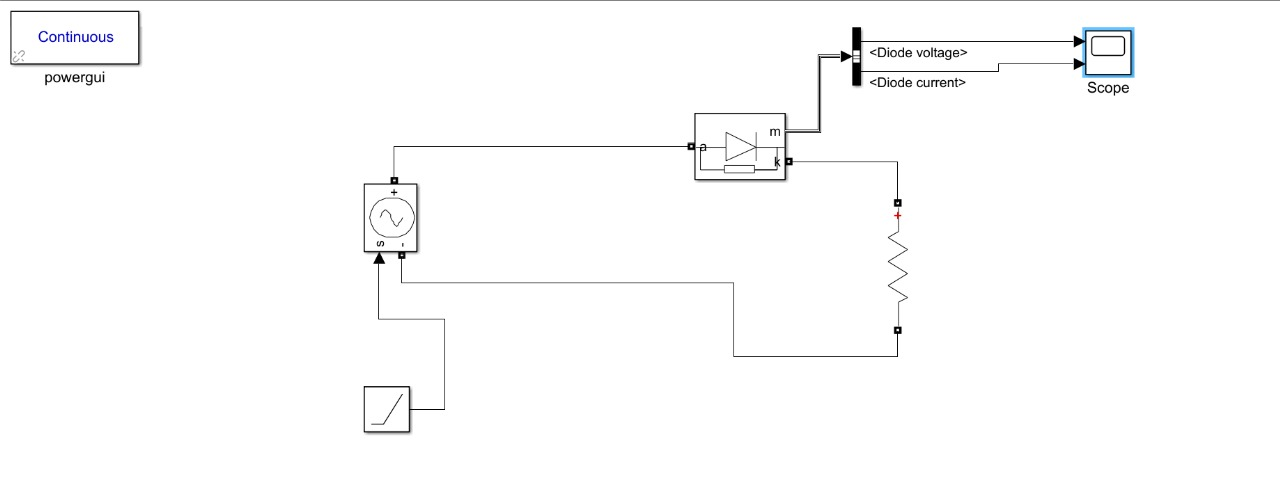
\includegraphics[width=0.8\textwidth]{Rdiag.jpg}
    \caption{Diode with Resistive Load}
    \label{fig:dc_r_load}
\end{figure}

\begin{figure}[H]
    \centering
    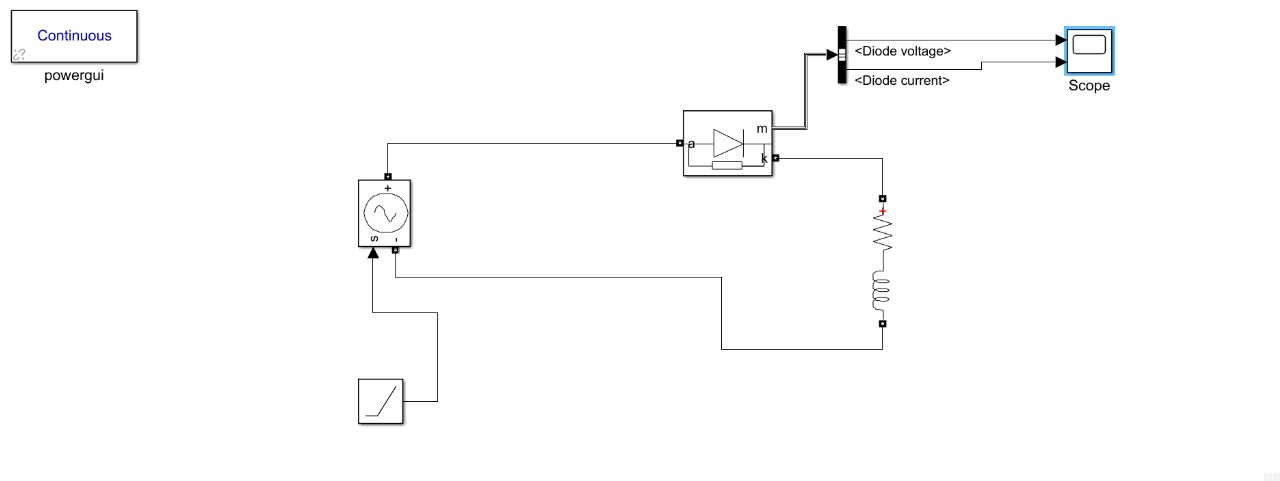
\includegraphics[width=0.8\textwidth]{RLdiag.jpg}
    \caption{Diode with Resistive-Inductive Load}
    \label{fig:dc_rl_load}
\end{figure}

\section*{Observations}
\addcontentsline{toc}{section}{Observations}
\begin{itemize}
    \item The diode conducts current in the forward bias and blocks current in the reverse bias.
    \item The diode exhibits rectification properties when connected to an AC supply.
    \item The load conditions (resistive, inductive) affect the diode's behavior and the output waveform.
    \item The output waveform changes based on the load conditions and the applied voltage.
    \item The diode's characteristics can be analyzed using an oscilloscope and signal generator.
    \item The diode's threshold voltage, forward current, and reverse current can be measured using the oscilloscope.
    \item The diode's response to different input signals can be observed using the oscilloscope.
\end{itemize}
\subsubsection*{Outputs}
\begin{figure}[H]
    \centering
    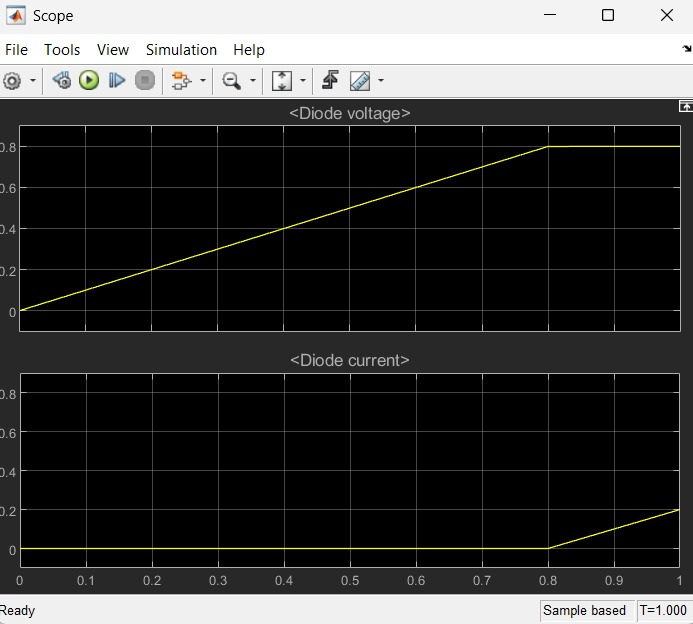
\includegraphics[width=0.6\textwidth]{Rwave.jpg}
    \caption{Simulation Diagram of Diode Circuit With R Load}
    \label{fig:simulation_diagram}
\end{figure}

\begin{figure}[H]
    \centering
    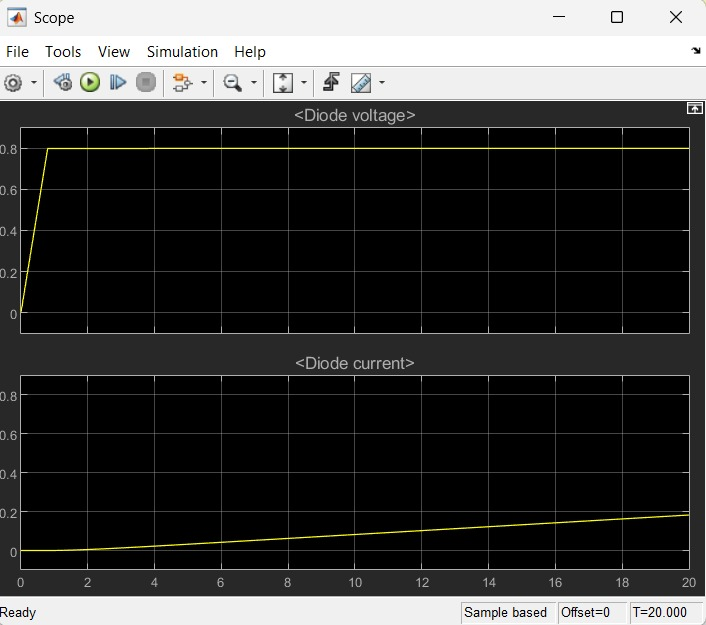
\includegraphics[width=0.6\textwidth]{RLwave.jpg}
    \caption{Oscilloscope Output for Forward Bias With RL Load}
    \label{fig:scope_forward_bias}
\end{figure}

\begin{figure}[H]
    \centering
    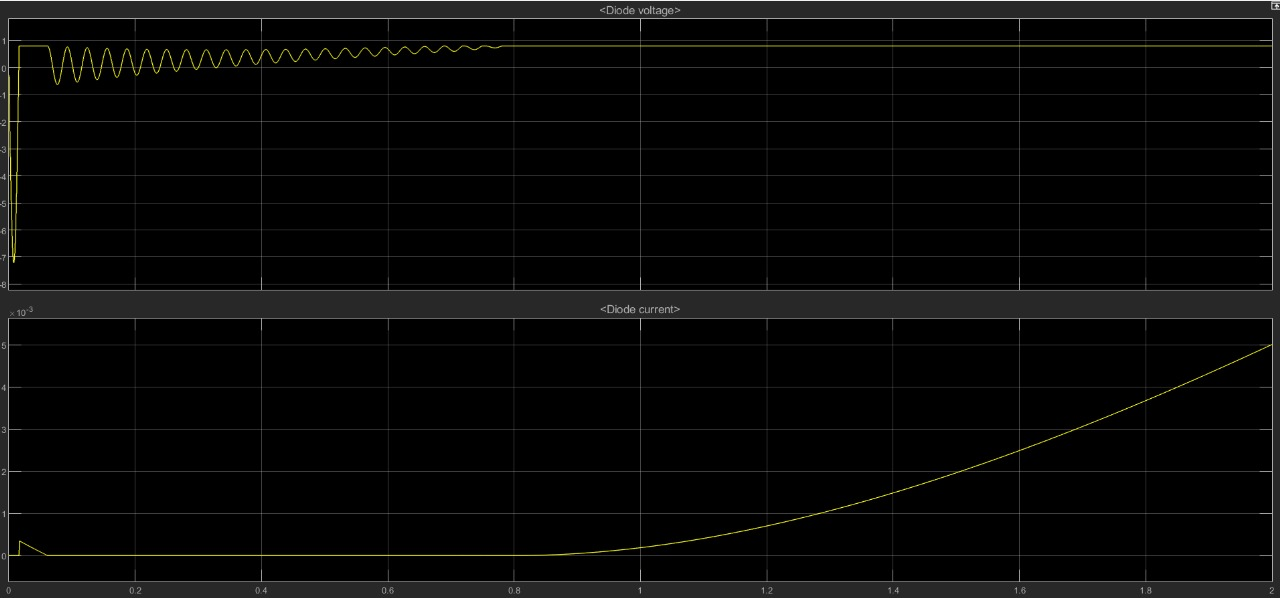
\includegraphics[width=0.6\textwidth]{RLwave2.jpg}
    \caption{Oscilloscope Output for RL Load}
    \label{fig:scope_reverse_bias}
\end{figure}


\section*{Discussion}
\addcontentsline{toc}{section}{Discussion}
The experiment demonstrates the diode's behavior under different load conditions and supply voltages. The diode's characteristics, such as forward bias, reverse bias, and rectification properties, are observed using simulation software. The oscilloscope and signal generator help visualize the diode's response to various input signals and load conditions. The experiment provides insights into the diode's operation and its applications in electronic circuits.

\section*{Conclusion}
\addcontentsline{toc}{section}{Conclusion}
The experiment explores the characteristics of a diode under different load conditions using DC and AC supplies. The diode's behavior in forward bias, reverse bias, and rectification is observed using simulation software. The oscilloscope and signal generator help analyze the diode's response to various input signals and load conditions. The experiment enhances understanding of the diode's operation and its applications in electronic circuits.

\bibliographystyle{IEEEtran}
\renewcommand{\bibname}{References}
\addcontentsline{toc}{section}{References}
\bibliography{ref}

\end{document}
